\chapter{Curves}\label{chap:curves}

微分几何研究的是曲线和曲面的几何性质。与微积分研究函数变化不同，微分几何研究空间中曲线和曲面的"形状"——弯曲程度、扭曲程度等内在几何量。

% ==================== Section 1-1: Introduction ====================
\section{Introduction}\label{sec:intro}

微分几何有两个基本方面。一种可称为\textbf{经典微分几何}，它始于微积分诞生之时。粗略地说，经典微分几何研究曲线和曲面的\textbf{局部性质}（local properties）。所谓局部性质，是指那些仅依赖于曲线或曲面在一点附近行为的几何性质。研究这种性质所使用的主要工具是微分计算。因此，微分几何中研究的曲线和曲面是由可微函数定义的。

另一种是\textbf{整体微分几何}（global differential geometry）。这里我们研究局部几何性质如何影响整条曲线或整个曲面的行为。本书后面会回到这个方面。

或许经典微分几何中最有趣且最具代表性的部分是曲面的研究。然而，在研究曲面时，曲线的某些局部性质会自然出现。因此，我们用这第一章来简要处理曲线理论。

\begin{Remark}
本章的组织方式使得只想学习曲面的读者可以只阅读 1-2 节到 1-5 节。
\begin{itemize}
\item 1-2 节到 1-4 节包含基础内容（参数曲线、弧长、向量积），这些内容在其他课程中可能已经学过，这里仅作复习；
\item 1-5 节是本章的核心，包含学习曲面所需的曲线理论；
\item 1-6 节和 1-7 节是可选的进一步内容。
\end{itemize}
\end{Remark}

% ==================== Section 1-2: Parametrized Curves ====================
\section{Parametrized Curves}\label{sec:parametrized-curves}

\begin{Remark}
接下来我们简要回顾 $\mathbb{R}^3$ 中向量内积的性质。设 $u = (u_1, u_2, u_3) \in \mathbb{R}^3$，定义其范数（或长度）为
\[
|u| = \sqrt{u_1^2 + u_2^2 + u_3^2}.
\]
几何上，$|u|$ 是点 $(u_1, u_2, u_3)$ 到原点 $O = (0, 0, 0)$ 的距离。

设 $u = (u_1, u_2, u_3)$ 和 $v = (v_1, v_2, v_3)$ 是 $\mathbb{R}^3$ 中的向量，$\theta$ ($0 \leq \theta \leq \pi$) 是线段 $Ou$ 和 $Ov$ 之间的夹角。内积 $u \cdot v$ 定义为（见教材 Figure 1-6）：
\[
u \cdot v = |u| |v| \cos\theta.
\]

内积的基本性质：
\begin{enumerate}
\item 若 $u$ 和 $v$ 为非零向量，则 $u \cdot v = 0$ 当且仅当 $u$ 与 $v$ 正交；
\item $u \cdot v = v \cdot u$；
\item $\lambda(u \cdot v) = \lambda u \cdot v = u \cdot \lambda v$；
\item $u \cdot (v + w) = u \cdot v + u \cdot w$。
\end{enumerate}
\end{Remark}

\begin{figure}[H]
\centering
\begin{minipage}{0.7\textwidth}
\centering
\subfloat[Figure 1-6. 内积的几何意义]{\label{fig:fig1-6}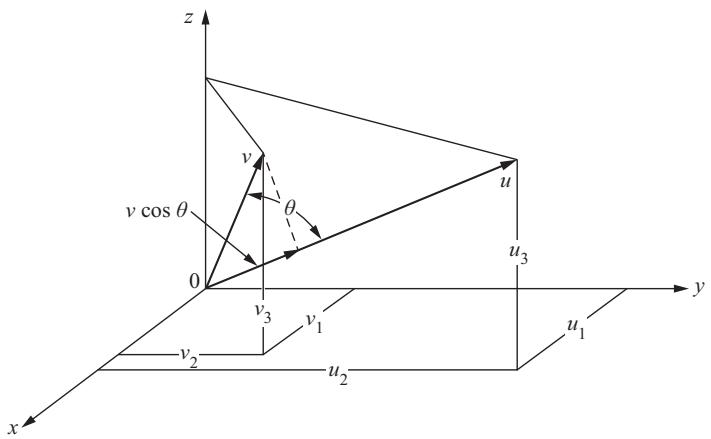
\includegraphics[width=\textwidth]{../../../../PDFs/differential-geometry/transcript/Do Carmo - Differential Geometry of Curves and Surfaces/hybrid_ocr/images/a0b92278a00bbcb50d6fd77bfcf8714675cdfc630be2b734b1bf7849214de53e.jpg}}
\end{minipage}
\end{figure}

我们用 $\mathbb{R}^3$ 表示所有三元实数有序组 $(x, y, z)$ 的集合。我们的目标是刻画 $\mathbb{R}^3$ 的某些子集（称为\textbf{曲线}），它们在某种意义上是一维的，并且微积分的方法可以应用其上。定义这种子集的一种自然方式是通过可微函数。

\begin{Definition}[可微参数曲线]\label{def:parametrized-curve}
\textbf{可微参数曲线}是一个可微映射
\[
\alpha: \mathbf{I} \to \mathbb{R}^3,
\]
其中 $\mathbf{I} = (\mathbf{a}, \mathbf{b})$ 是实数直线 $\mathbb{R}$ 上的一个开区间。
\end{Definition}

可微意味着 $\alpha$ 将每个 $t \in I$ 映射到点 $\alpha(t) = (x(t), y(t), z(t)) \in \mathbb{R}^3$，其中函数 $x(t), y(t), z(t)$ 都是可微的。变量 $t$ 称为曲线的\textbf{参数}。

如果记 $x(t)$ 在 $t$ 处的一阶导数为 $x'(t)$，等等，则向量
\[
(x'(t), y'(t), z'(t)) = \alpha'(t) \in \mathbb{R}^3
\]
称为曲线 $\alpha$ 在 $t$ 处的\textbf{切向量}（tangent vector）或\textbf{速度向量}（velocity vector）。像集 $\alpha(I) \subset \mathbb{R}^3$ 称为 $\alpha$ 的\textbf{迹}（trace）。如下面的例 5 所示，我们必须注意区分参数曲线（它是一个映射）和它的迹（它是 $\mathbb{R}^3$ 的一个子集）。

\begin{Remark}
术语说明：许多人用"无限可微"来表示具有各阶导数（且自动连续）的函数，而用"可微"仅表示一阶导数的存在性。我们不采用这种用法——本书中"可微"意味着所有阶导数都存在。
\end{Remark}

\begin{figure}[H]
\centering
\begin{minipage}{0.30\textwidth}
\centering
\subfloat[Figure 1-1. 圆柱螺旋线 (helix)]{\label{fig:helix}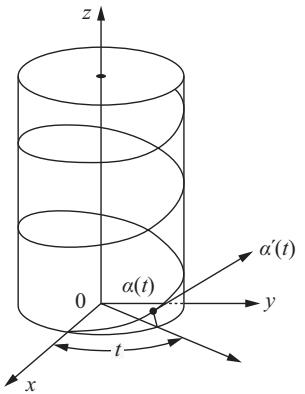
\includegraphics[width=\textwidth]{../../../../PDFs/differential-geometry/transcript/Do Carmo - Differential Geometry of Curves and Surfaces/hybrid_ocr/images/1368896b0e1df27036554e8c66d6bc05c3fbc6b6c2bca19cecb0d396544dfb0a.jpg}}
\end{minipage}
\hfill
\begin{minipage}{0.35\textwidth}
\centering
\subfloat[Figure 1-2. 奇异点例子]{\label{fig:trace1}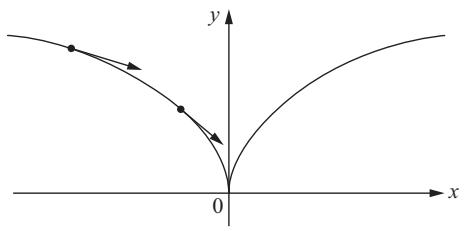
\includegraphics[width=\textwidth]{../../../../PDFs/differential-geometry/transcript/Do Carmo - Differential Geometry of Curves and Surfaces/hybrid_ocr/images/fe1d17628a3c9bb1e6afbeeae0fdac47edd92f0cb4651af800c230be43509433.jpg}}
\newline
\subfloat[Figure 1-3. 非单射曲线例子]{\label{fig:trace2}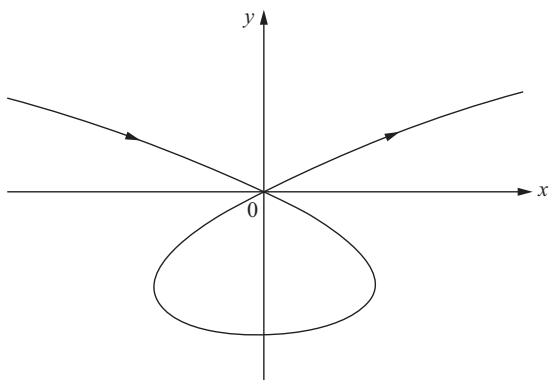
\includegraphics[width=\textwidth]{../../../../PDFs/differential-geometry/transcript/Do Carmo - Differential Geometry of Curves and Surfaces/hybrid_ocr/images/cb0e93ccd913afbcf8adab5178a99f0ac4808db3b32ad2dbe4971ce9b314a9aa.jpg}}
\end{minipage}
\end{figure}

\begin{Example}[圆柱螺旋线]\label{ex:helix}
参数方程
\[
\alpha(t) = (a\cos t,\; a\sin t,\; bt),\quad t \in \mathbb{R}
\]
在 $\mathbb{R}^3$ 中的迹是圆柱面 $x^2 + y^2 = a^2$ 上的螺旋线（helix），螺距（pitch）为 $2\pi b$。这里参数 $t$ 测量的是 $x$ 轴与从原点 $O$ 到点 $\alpha(t)$ 在 $xy$ 平面上投影点的连线之间的夹角（见教材 Figure 1-1）。
\end{Example}

\begin{Example}[奇异点]\label{ex:singular-point}
映射 $\alpha: \mathbb{R} \to \mathbb{R}^2$，$\alpha(t) = (t^3, t^2)$，是一条可微参数曲线（见教材 Figure 1-2）。注意 $\alpha'(0) = (0, 0)$——即 $t = 0$ 处的速度向量为零。这样的点称为\textbf{奇异点}（singular point）。
\end{Example}

\begin{Example}[非单射曲线]\label{ex:non-injective}
映射 $\alpha: \mathbb{R} \to \mathbb{R}^2$，$\alpha(t) = (t^3 - 4t,\; t^2 - 4)$，是一条可微参数曲线（见教材 Figure 1-3）。注意 $\alpha(2) = \alpha(-2) = (0, 0)$——即映射 $\alpha$ 不是单射。
\end{Example}

\begin{Example}[不可微曲线]\label{ex:nondifferentiable}
映射 $\alpha: \mathbb{R} \to \mathbb{R}^2$，$\alpha(t) = (t, |t|)$，$t \in \mathbb{R}$，不是可微参数曲线，因为 $|t|$ 在 $t = 0$ 处不可微（见教材 Figure 1-4）。
\end{Example}

\begin{figure}[H]
\centering
\begin{minipage}{0.55\textwidth}
\centering
\subfloat[Figure 1-4. 不可微曲线 $(t, |t|)$]{\label{fig:fig1-4}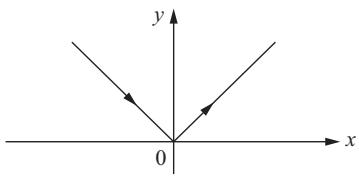
\includegraphics[width=\textwidth]{../../../../PDFs/differential-geometry/transcript/Do Carmo - Differential Geometry of Curves and Surfaces/hybrid_ocr/images/3ccb4fd7f5ebe66c541905ee2202d214dc1c8d2d699dace1fe66d0754f0bba7d.jpg}}
\end{minipage}
\hfill
\begin{minipage}{0.40\textwidth}
\centering
\subfloat[Figure 1-5. 相同圆的不同参数化]{\label{fig:fig1-5}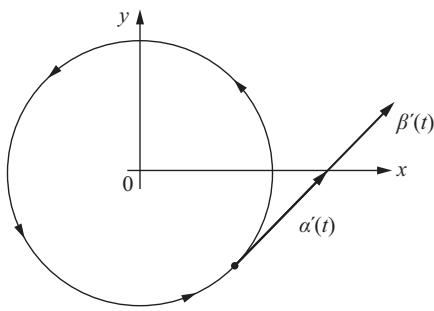
\includegraphics[width=\textwidth]{../../../../PDFs/differential-geometry/transcript/Do Carmo - Differential Geometry of Curves and Surfaces/hybrid_ocr/images/5c1a7770e5c0b4bfc9eab7055561b6a0abd1f5782eb7ecbdebd9abcbd5977fe3.jpg}}
\end{minipage}
\end{figure}

\begin{Example}[相同迹的不同参数化]\label{ex:same-trace-different-param}
两条不同的参数曲线
\[
\alpha(t) = (\cos t, \sin t),\quad \beta(t) = (\cos 2t, \sin 2t),
\]
其中 $t \in (-\epsilon, 2\pi + \epsilon)$，$\epsilon > 0$，具有相同的迹——即单位圆 $x^2 + y^2 = 1$。但第二条曲线的速度向量是第一条的两倍（见教材 Figure 1-5）。
\end{Example}

\subsection*{1-2 节练习}

\begin{exercise}{1-2, 1}
Find a parametrized curve $\alpha(t)$ whose trace is the circle $x^2 + y^2 = 1$ such that $\alpha(t)$ runs clockwise around the circle with $\alpha(0) = (0, 1)$.
\end{exercise}

\begin{exercise}{1-2, 2}
Let $\alpha(t)$ be a parametrized curve which does not pass through the origin. If $\alpha(t_0)$ is a point of the trace of $\alpha$ closest to the origin and $\alpha'(t_0) \neq 0$, show that the position vector $\alpha(t_0)$ is orthogonal to $\alpha'(t_0)$.
\end{exercise}

\begin{exercise}{1-2, 3}
A parametrized curve $\alpha(t)$ has the property that its second derivative $\alpha''(t)$ is identically zero. What can be said about $\alpha$?
\end{exercise}

\begin{exercise}{1-2, 4}
Let $\alpha: I \to \mathbb{R}^3$ be a parametrized curve and let $v \in \mathbb{R}^3$ be a fixed vector. Assume that $\alpha'(t)$ is orthogonal to $v$ for all $t \in I$ and that $\alpha(0)$ is also orthogonal to $v$. Prove that $\alpha(t)$ is orthogonal to $v$ for all $t \in I$.
\end{exercise}

\begin{exercise}{1-2, 5}
Let $\alpha: I \to \mathbb{R}^3$ be a parametrized curve, with $\alpha'(t) \neq 0$ for all $t \in I$. Show that $|\alpha(t)|$ is a nonzero constant if and only if $\alpha(t)$ is orthogonal to $\alpha'(t)$ for all $t \in I$.
\end{exercise}

% ==================== Section 1-3: Regular Curves; Arc Length ====================
\section{Regular Curves; Arc Length}\label{sec:regular-arc-length}

设 $\alpha: I \to \mathbb{R}^3$ 是一条可微参数曲线。对于每个满足 $\alpha'(t) \neq 0$ 的 $t \in I$，存在一条唯一定义直线，它经过点 $\alpha(t)$ 且与向量 $\alpha'(t)$ 平行。这条直线称为曲线 $\alpha$ 在 $t$ 处的\textbf{切线}（tangent line）。因此，研究曲线的微分几何时，关键是每一点都存在这样的切线。于是我们把 $\alpha'(t) = 0$ 的点称为 $\alpha$ 的\textbf{奇异点}（singular point），并把注意力限制在没有奇异点的曲线上。注意例 2 中 $t = 0$ 就是一个奇异点。

\begin{Definition}[正则曲线]\label{def:regular-curve}
如果 $\alpha'(t) \neq 0$ 对所有 $t \in \mathbf{I}$ 成立，则称可微参数曲线 $\alpha: \mathbf{I} \to \mathbb{R}^3$ 为\textbf{正则曲线}（regular curve）。
\end{Definition}

现在考虑曲线的长度概念。

\begin{Definition}[弧长]\label{def:arc-length}
设 $\alpha: [a,b] \to \mathbb{R}^3$ 是一条可微曲线。$\alpha$ 从 $t = a$ 到 $t$ 的\textbf{弧长}（arc length）定义为
\[
s(t) = \int_a^t \|\alpha'(u)\| \, du.
\]
\end{Definition}

弧长是曲线的内在不变量，与参数化选择无关。

\begin{figure}[H]
\centering
\begin{minipage}{0.85\textwidth}
\centering
\subfloat[Figure 1-7. 旋轮线 (cycloid)]{\label{fig:cycloid}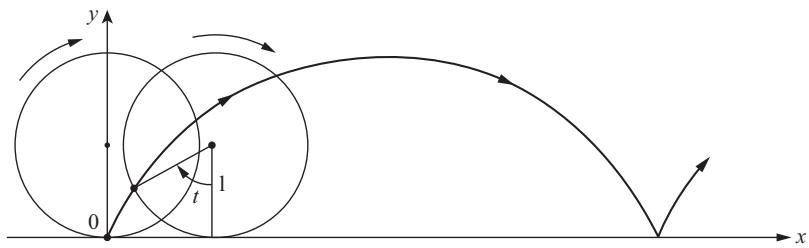
\includegraphics[width=\textwidth]{../../../../PDFs/differential-geometry/transcript/Do Carmo - Differential Geometry of Curves and Surfaces/hybrid_ocr/images/63bc08d607172bd6a8b21cbb1b3d77d9488cb451250e9185505320fee946bdea.jpg}}
\end{minipage}
\end{figure}

\begin{figure}[H]
\centering
\begin{minipage}{0.35\textwidth}
\centering
\subfloat[Figure 1-8. Diocles 割舌线 (cissoid)]{\label{fig:cissoid}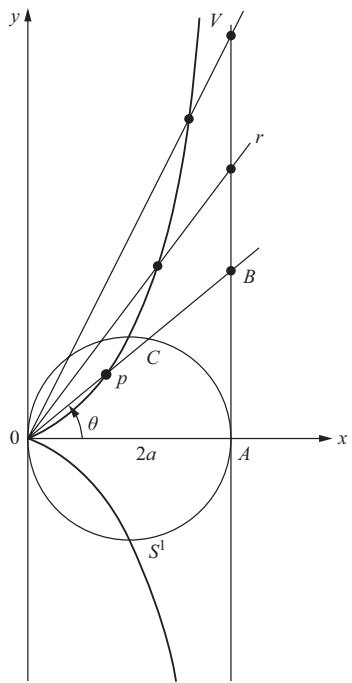
\includegraphics[width=\textwidth]{../../../../PDFs/differential-geometry/transcript/Do Carmo - Differential Geometry of Curves and Surfaces/hybrid_ocr/images/7cb4e48e7dffd2801d004ed55334f427682431254e840be3a0f41770ff7e5f4b.jpg}}
\end{minipage}
\hfill
\begin{minipage}{0.30\textwidth}
\centering
\subfloat[Figure 1-9. 曳物线 (tractrix)]{\label{fig:tractrix}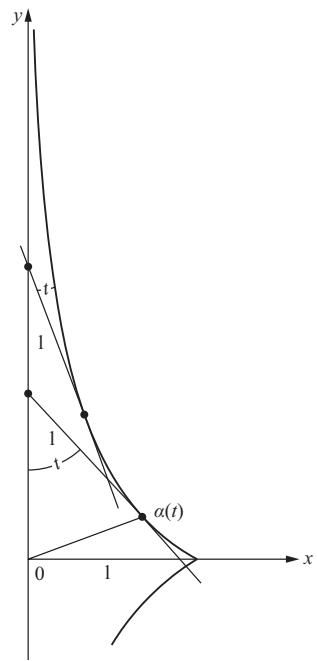
\includegraphics[width=\textwidth]{../../../../PDFs/differential-geometry/transcript/Do Carmo - Differential Geometry of Curves and Surfaces/hybrid_ocr/images/ce65cd4c5b99c388091efe63d303bf387148984fd4d56aa49e7df3e7ecee7b8b.jpg}}
\end{minipage}
\end{figure}

\begin{Proposition}[弧长参数化]\label{prop:arc-length-reparam}
设 $\alpha: I \to \mathbb{R}^3$ 是正则曲线。定义
\[
s(t) = \int_{t_0}^t \|\alpha'(u)\| \, du,
\]
其中 $t_0 \in I$ 是固定点。由于 $\alpha$ 是正则的，$s'(t) = \|\alpha'(t)\| > 0$，所以 $s$ 是严格递增的，可以取逆函数 $t(s)$。则 $\beta(s) = \alpha(t(s))$ 是单位速度曲线。
\end{Proposition}

\begin{Definition}[单位速度曲线]\label{def:unit-speed}
如果 $\|\alpha'(t)\| = 1$ 对所有 $t$ 成立，则称 $\alpha$ 为\textbf{单位速度曲线}（unit speed curve）或\textbf{弧长参数化曲线}。
\end{Definition}

从现在开始，除非特别说明，我们将使用弧长 $s$ 作为参数，即 $\alpha(s)$ 是单位速度曲线。

\begin{Remark}
弧长参数化后，速度向量恒为 $1$，这是最自然的参数化方式。此时 $\alpha'(s)$ 是单位切向量。
\end{Remark}

\begin{Example}[圆的弧长]\label{ex:circle-arc-length}
半径为 $a$ 的圆可以参数化为 $\alpha(t) = (a\cos t, a\sin t, 0)$，$t \in [0, 2\pi]$。则弧长
\[
s(t) = \int_0^t \|\alpha'(u)\| \, du = \int_0^t a \, du = at,
\]
所以从 $t = 0$ 到 $t = 2\pi$ 的全长是 $2\pi a$。
\end{Example}

\begin{Example}[圆柱螺旋线的弧长]\label{ex:helix-arc-length}
圆柱螺旋线 $\alpha(t) = (a\cos t, a\sin t, bt)$ 的速度向量为 $\alpha'(t) = (-a\sin t, a\cos t, b)$，模长为
\[
\|\alpha'(t)\| = \sqrt{a^2 + b^2}.
\]
因此弧长为 $s(t) = \sqrt{a^2 + b^2}\, t$。
\end{Example}

\begin{figure}[H]
\centering
\begin{minipage}{0.45\textwidth}
\centering
\subfloat[Figure 1-10. 笛卡尔叶形线 (folium of Descartes)]{\label{fig:folium}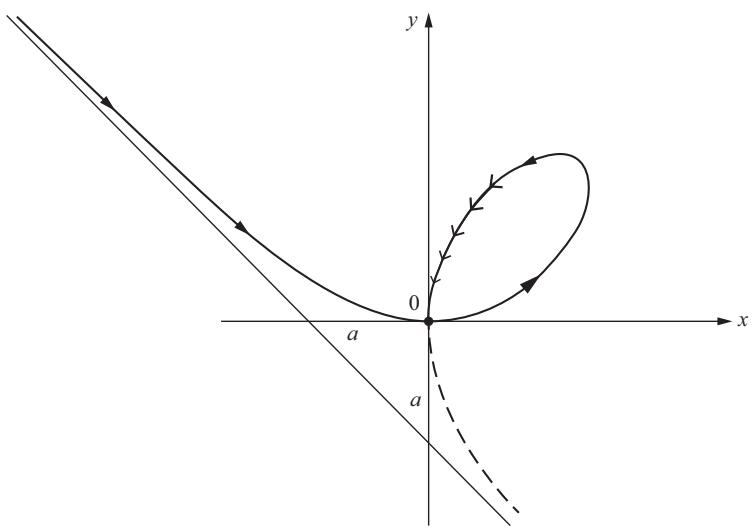
\includegraphics[width=\textwidth]{../../../../PDFs/differential-geometry/transcript/Do Carmo - Differential Geometry of Curves and Surfaces/hybrid_ocr/images/53989c2c8bd35e9940d7e50e2d083d788a381c25ec567919134018f0aa652a4a.jpg}}
\end{minipage}
\hfill
\begin{minipage}{0.45\textwidth}
\centering
\subfloat[Figure 1-11. 对数螺旋线 (logarithmic spiral)]{\label{fig:log-spiral}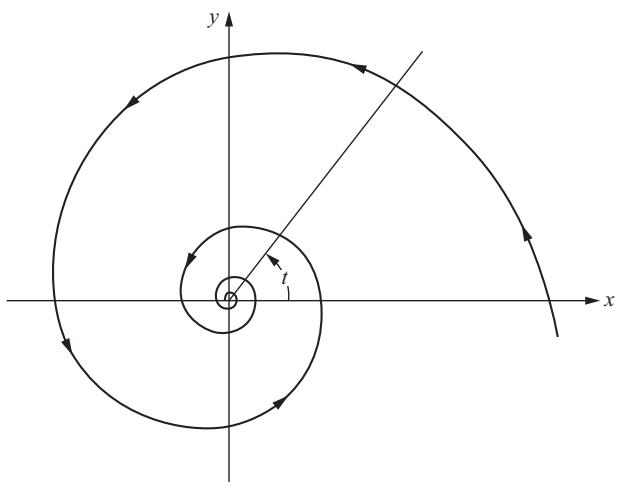
\includegraphics[width=\textwidth]{../../../../PDFs/differential-geometry/transcript/Do Carmo - Differential Geometry of Curves and Surfaces/hybrid_ocr/images/2174ba1ba51fc162114661ee328aff35710e3764b7c59adb18400b0b6598d634.jpg}}
\end{minipage}
\end{figure}

\subsection*{1-3 节练习}

\begin{exercise}{1-3, 1}
Show that the tangent lines to the regular parametrized curve $\alpha(t) = (3t, 3t^2, 2t^3)$ make a constant angle with the line $y = 0,\; z = x$.
\end{exercise}

\begin{exercise}{1-3, 2}
A circular disk of radius 1 in the plane $xy$ rolls without slipping along the $x$ axis. The figure described by a point of the circumference of the disk is called a cycloid (见教材 Figure 1-7)。
\begin{enumerate}
\item[a.] Obtain a parametrized curve $\alpha: \mathbb{R} \to \mathbb{R}^2$ the trace of which is the cycloid, and determine its singular points.
\item[b.] Compute the arc length of the cycloid corresponding to a complete rotation of the disk.
\end{enumerate}
\end{exercise}

\begin{exercise}{1-3, 3}
Let $0A = 2a$ be the diameter of a circle $S^1$. Prove that:
\begin{enumerate}
\item[a.] The trace of $\alpha(t) = \left(\frac{2at^2}{1+t^2}, \frac{2at^3}{1+t^2}\right)$, $t \in \mathbb{R}$, is the cissoid of Diocles (见教材 Figure 1-8).
\item[b.] The origin $(0,0)$ is a singular point of the cissoid.
\item[c.] As $t \to \infty$, $\alpha(t)$ approaches the line $x = 2a$ (asymptote).
\end{enumerate}
\end{exercise}

\begin{exercise}{1-3, 4}
Let $\alpha: (0, \pi) \to \mathbb{R}^2$ be given by $\alpha(t) = \left(\sin t, \cos t + \log \tan \frac{t}{2}\right)$. The trace of $\alpha$ is called the tractrix (见教材 Figure 1-9). Show that:
\begin{enumerate}
\item[a.] $\alpha$ is a differentiable parametrized curve, regular except at $t = \pi/2$.
\item[b.] The length of the segment of the tangent of the tractrix between the point of tangency and the $y$ axis is constantly equal to $1$.
\end{enumerate}
\end{exercise}

% ==================== Section 1-4: The Vector Product in R3 ====================
\section{The Vector Product in $\mathbb{R}^3$}\label{sec:vector-product-ch1}

向量积（或叉积、外积）是 $\mathbb{R}^3$ 中特有的运算，在曲线与曲面的理论中起关键作用。

\begin{Definition}[向量积]\label{def:cross-product-ch1}
设 $\mathbf{u} = (u_1, u_2, u_3)$ 和 $\mathbf{v} = (v_1, v_2, v_3)$ 是 $\mathbb{R}^3$ 中的向量。定义\textbf{向量积}（cross product）$\mathbf{u} \times \mathbf{v} \in \mathbb{R}^3$ 为
\[
\mathbf{u} \times \mathbf{v} = (u_2 v_3 - u_3 v_2,\; u_3 v_1 - u_1 v_3,\; u_1 v_2 - u_2 v_1).
\]
向量积可以用行列式简洁地表示为
\[
\mathbf{u} \times \mathbf{v} = \det\begin{pmatrix}
\mathbf{e}_1 & \mathbf{e}_2 & \mathbf{e}_3 \\
u_1 & u_2 & u_3 \\
v_1 & v_2 & v_3
\end{pmatrix}.
\]
\end{Definition}

向量积的基本性质：

\begin{Proposition}[向量积的性质]\label{prop:cross-product-ch1}
设 $\mathbf{u}, \mathbf{v}, \mathbf{w} \in \mathbb{R}^3$，$\lambda \in \mathbb{R}$，则：
\begin{enumerate}
\item（反交换律）$\mathbf{u} \times \mathbf{v} = -\mathbf{v} \times \mathbf{u}$；
\item（数乘结合律）$(\lambda \mathbf{u}) \times \mathbf{v} = \lambda (\mathbf{u} \times \mathbf{v}) = \mathbf{u} \times (\lambda \mathbf{v})$；
\item（分配律）$\mathbf{u} \times (\mathbf{v} + \mathbf{w}) = \mathbf{u} \times \mathbf{v} + \mathbf{u} \times \mathbf{w}$；
\item（标量三重积）$(\mathbf{u} \times \mathbf{v}) \cdot \mathbf{w} = \det(\mathbf{u}, \mathbf{v}, \mathbf{w})$。
\end{enumerate}
\end{Proposition}

向量积的几何意义：

\begin{Proposition}[向量积的几何意义]\label{prop:cross-product-geometry-ch1}
\begin{enumerate}
\item $\mathbf{u} \times \mathbf{v}$ 垂直于 $\mathbf{u}$ 和 $\mathbf{v}$ 所在的平面；
\item $\mathbf{u} \times \mathbf{v}$ 的方向由右手定则确定；
\item $\|\mathbf{u} \times \mathbf{v}\| = \|\mathbf{u}\| \|\mathbf{v}\| \sin\theta$，其中 $\theta$ 是 $\mathbf{u}$ 和 $\mathbf{v}$ 之间的夹角；
\item $\mathbf{u} \times \mathbf{v} = \mathbf{0}$ 当且仅当 $\mathbf{u}$ 和 $\mathbf{v}$ 平行。
\end{enumerate}
\end{Proposition}

\begin{figure}[H]
\centering
\begin{minipage}{0.6\textwidth}
\centering
\subfloat[Figure 1-13. 向量积几何意义]{\label{fig:cross-product-ch1}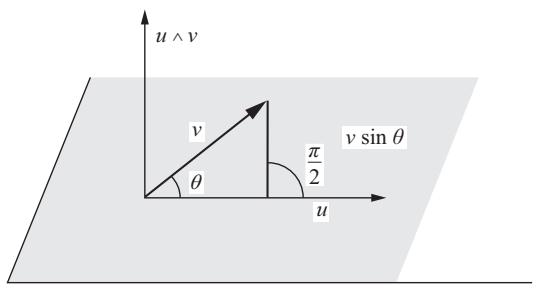
\includegraphics[width=\textwidth]{../../../../PDFs/differential-geometry/transcript/Do Carmo - Differential Geometry of Curves and Surfaces/hybrid_ocr/images/184a2a5cb54f57e8b0095aa8826470f2b433badc9f4dadb5c5fb24d76ad02bd1.jpg}}
\end{minipage}
\end{figure}

\begin{Remark}
向量积在曲线理论中的应用：
\begin{itemize}
\item 构造副法向量：$\mathbf{b} = \mathbf{t} \times \mathbf{n}$
\item 计算挠率：$\tau = \dfrac{\det(\alpha', \alpha'', \alpha''')}{k^2}$
\end{itemize}
\end{Remark}

\begin{figure}[H]
\centering
\begin{minipage}{0.6\textwidth}
\centering
\subfloat[Figure 1-12. 弧长逼近的几何意义]{\label{fig:arc-length-approx}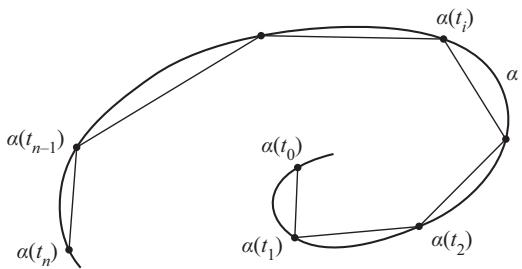
\includegraphics[width=\textwidth]{../../../../PDFs/differential-geometry/transcript/Do Carmo - Differential Geometry of Curves and Surfaces/hybrid_ocr/images/a9b16e888308f3816e421a0b7d3bfe30d5b264884d0cead14690e87b887aef3e.jpg}}
\end{minipage}
\end{figure}

% ==================== Section 1-5: The Local Theory of Curves ====================
\section{The Local Theory of Curves Parametrized by Arc Length}\label{sec:local-theory-ch1}

这是曲线理论的核心部分。我们将看到曲线的形状完全由两个函数决定：曲率（curvature）和挠率（torsion）。

\subsection{The Curvature}\label{sec:curvature}

\begin{Definition}[曲率]\label{def:curvature-ch1}
设 $\alpha(s)$ 是单位速度曲线。定义\textbf{曲率}（curvature）为
\[
k(s) = \|\alpha''(s)\|.
\]
即加速度向量的模长。
\end{Definition}

\begin{Remark}
曲率描述曲线弯曲的程度：
\begin{itemize}
\item 直线：曲率为 $0$，完全不弯曲；
\item 圆：曲率为常数 $1/a$（$a$ 为半径），弯曲程度均匀；
\item 曲率越大，曲线弯曲越厉害。
\end{itemize}
\end{Remark}

\begin{figure}[H]
\centering
\begin{minipage}{0.6\textwidth}
\centering
\subfloat[Figure 1-14. 曲率的几何意义]{\label{fig:curvature-geom}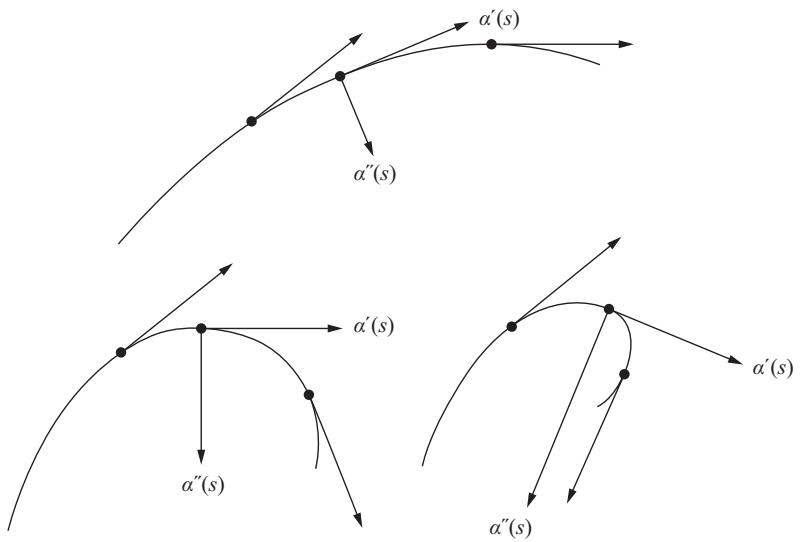
\includegraphics[width=\textwidth]{../../../../PDFs/differential-geometry/transcript/Do Carmo - Differential Geometry of Curves and Surfaces/hybrid_ocr/images/1aaf7d0d16f921f25b0f42575a0f8c844242e11985ae269a55e18b4acf7ad5b1.jpg}}
\end{minipage}
\end{figure}

\begin{Example}[圆的曲率]\label{ex:circle-curvature-ch1}
单位圆的参数方程 $\alpha(s) = (\cos s, \sin s, 0)$，则
\[
\alpha'(s) = (-\sin s, \cos s, 0),\quad \alpha''(s) = (-\cos s, -\sin s, 0),
\]
所以 $k(s) = \|\alpha''(s)\| = 1$。更一般地，半径为 $a$ 的圆的曲率为 $1/a$。
\end{Example}

\begin{Example}[直线的曲率]\label{ex:line-curvature-ch1}
直线 $\alpha(s) = \mathbf{p} + \mathbf{v}s$（$\mathbf{v}$ 为单位向量），则 $\alpha''(s) = 0$，所以 $k(s) = 0$。
\end{Example}

\begin{Definition}[主法向量]\label{def:principal-normal}
设 $\alpha(s)$ 是单位速度曲线，$k(s) > 0$。定义\textbf{主法向量}（principal normal）为
\[
\mathbf{n}(s) = \frac{\alpha''(s)}{k(s)} = \frac{\alpha''(s)}{\|\alpha''(s)\|}.
\]
\end{Definition}

\begin{Proposition}[曲率的另一个表达式]\label{prop:curvature-alternative}
设 $\alpha(t)$ 是正则曲线（不一定单位速度），则
\[
k(t) = \frac{\|\alpha'(t) \times \alpha''(t)\|}{\|\alpha'(t)\|^3}.
\]
\end{Proposition}

\subsection{The Torsion (Or Bending)}\label{sec:torsion}

挠率描述曲线"离开"所在平面的程度。

\begin{Definition}[挠率]\label{def:torsion-ch1}
设 $\alpha(s)$ 是单位速度曲线，假设 $k(s) > 0$。定义\textbf{挠率}（torsion）为
\[
\tau(s) = \frac{\det(\alpha'(s), \alpha''(s), \alpha'''(s))}{k(s)^2}.
\]
\end{Definition}

\begin{Remark}
挠率描述曲线在空间中的扭曲程度：
\begin{itemize}
\item 平面曲线：挠率恒为零（因为 $\alpha', \alpha'', \alpha'''$ 共面）；
\item 空间曲线：挠率可能非零，描述曲线"扭转"的程度。
\end{itemize}
\end{Remark}

\begin{Example}[圆柱螺旋线的挠率]\label{ex:helix-torsion-ch1}
圆柱螺旋线 $\alpha(t) = (a\cos t, a\sin t, bt)$ 的曲率为 $k = \dfrac{a}{a^2+b^2}$，挠率为 $\tau = \dfrac{b}{a^2+b^2}$，两者均为常数。
\end{Example}

\begin{Proposition}[挠率的另一个表达式]\label{prop:torsion-alternative}
设 $\alpha(s)$ 是单位速度曲线，$k(s) > 0$，则
\[
\tau(s) = -\langle \mathbf{b}'(s), \mathbf{n}(s) \rangle,
\]
其中 $\mathbf{b}(s) = \mathbf{t}(s) \times \mathbf{n}(s)$ 是副法向量。
\end{Proposition}

\begin{figure}[H]
\centering
\begin{minipage}{0.6\textwidth}
\centering
\subfloat[Figure 1-15. 密切平面与 Frenet 标架]{\label{fig:osculating-plane}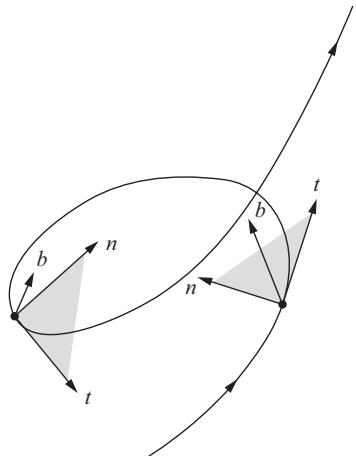
\includegraphics[width=\textwidth]{../../../../PDFs/differential-geometry/transcript/Do Carmo - Differential Geometry of Curves and Surfaces/hybrid_ocr/images/df17d953f8624c3870ca864e22d606bcf5467c6aa64274d0f56de41cb925f55b.jpg}}
\end{minipage}
\end{figure}

\subsection{The Frenet-Serret Formulas}\label{sec:frenet-serret}

Frenet-Serret 公式是微分几何中最重要的公式之一。

\begin{Definition}[Frenet 标架]\label{def:frenet-frame-ch1}
设 $\alpha(s)$ 是单位速度曲线，$k(s) > 0$。定义：
\begin{enumerate}
\item \textbf{切向量}（tangent vector）：$\mathbf{t}(s) = \alpha'(s)$；
\item \textbf{主法向量}（principal normal）：$\mathbf{n}(s) = \dfrac{\alpha''(s)}{k(s)}$；
\item \textbf{副法向量}（binormal）：$\mathbf{b}(s) = \mathbf{t}(s) \times \mathbf{n}(s)$。
\end{enumerate}
$\{\mathbf{t}, \mathbf{n}, \mathbf{b}\}$ 称为\textbf{Frenet 标架}（Frenet frame）。它们构成 $\mathbb{R}^3$ 的标准正交基（右手系）。
\end{Definition}

\begin{figure}[H]
\centering
\begin{minipage}{0.45\textwidth}
\centering
\subfloat[Figure 1-16 (a). 有向曲率 - 正向]{\label{fig:signed-curvature-pos}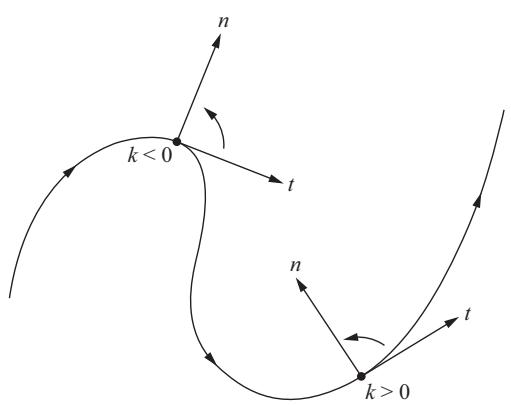
\includegraphics[width=\textwidth]{../../../../PDFs/differential-geometry/transcript/Do Carmo - Differential Geometry of Curves and Surfaces/hybrid_ocr/images/55c8df215ceffa70ad05761b78e5c57a32b3796d9d40e2914ae6e471b5f58de1.jpg}}
\end{minipage}
\hfill
\begin{minipage}{0.45\textwidth}
\centering
\subfloat[Figure 1-16 (b). 有向曲率 - 负向]{\label{fig:signed-curvature-neg}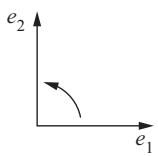
\includegraphics[width=\textwidth]{../../../../PDFs/differential-geometry/transcript/Do Carmo - Differential Geometry of Curves and Surfaces/hybrid_ocr/images/857b8e3e7e82e9d09b5e70dd850b1451dc6d837a1b5bdb42717a3c286dd929b6.jpg}}
\end{minipage}
\end{figure}

\begin{Definition}[密切平面、法平面、化直平面]\label{def:osculating-plane-ch1}
\begin{itemize}
\item \textbf{密切平面}（osculating plane）：由 $\mathbf{t}(s)$ 和 $\mathbf{n}(s)$ 张成的平面；
\item \textbf{法平面}（normal plane）：由 $\mathbf{n}(s)$ 和 $\mathbf{b}(s)$ 张成的平面；
\item \textbf{化直平面}（rectifying plane）：由 $\mathbf{t}(s)$ 和 $\mathbf{b}(s)$ 张成的平面。
\end{itemize}
\end{Definition}

\begin{Theorem}[Frenet-Serret 公式]\label{th:frenet-serret-ch1}
设 $\alpha(s)$ 是单位速度曲线，$k(s) > 0$，挠率为 $\tau(s)$。则
\[
\begin{cases}
\mathbf{t}' = k \mathbf{n}, \\
\mathbf{n}' = -k \mathbf{t} + \tau \mathbf{b}, \\
\mathbf{b}' = -\tau \mathbf{n}.
\end{cases}
\]
\end{Theorem}

\begin{Corollary}[曲率和挠率的计算]\label{cor:curvature-torsion-ch1}
曲率和挠率可以通过以下公式计算：
\[
k = \|\mathbf{t}'\|, \quad \tau = -\langle \mathbf{b}', \mathbf{n} \rangle.
\]
\end{Corollary}

\begin{Remark}
Frenet-Serret 公式表明，如果我们知道曲率 $k(s)$ 和挠率 $\tau(s)$，以及初始的 Frenet 标架，就可以唯一确定曲线的形状。这两个函数完全决定了曲线（在局部意义上）。这类似于刚体运动学：给定线速度和角速度，就能确定刚体的运动。
\end{Remark}

\begin{Theorem}[曲线存在唯一性定理]\label{th:curve-existence-ch1}
给定两个连续函数 $k(s) > 0$ 和 $\tau(s)$，以及 $\mathbb{R}^3$ 中一组正交标架，存在唯一一条单位速度曲线 $\alpha(s)$，使得其曲率为 $k(s)$、挠率为 $\tau(s)$，且 Frenet 标架为给定的标架。
\end{Theorem}

\begin{Remark}
这是微分几何中的一个基本存在唯一性定理。它告诉我们：曲率和挠率完全决定了曲线的形状。
\end{Remark}

\begin{figure}[H]
\centering
\begin{minipage}{0.6\textwidth}
\centering
\subfloat[Figure 1-17. 渐伸线 (evolute)]{\label{fig:evolute-ch1}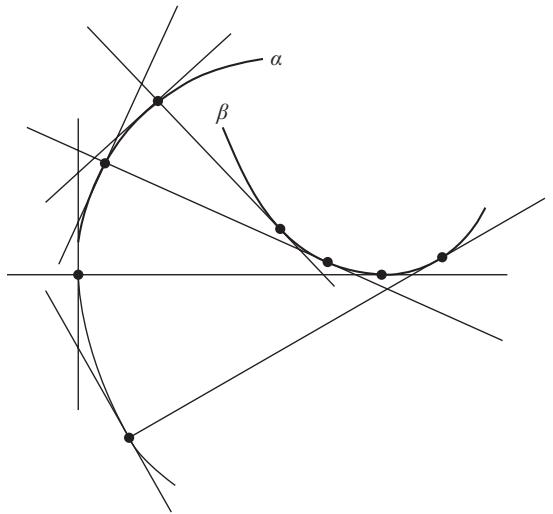
\includegraphics[width=\textwidth]{../../../../PDFs/differential-geometry/transcript/Do Carmo - Differential Geometry of Curves and Surfaces/hybrid_ocr/images/85b70efc49d0cda9439f1c08272dfd6fec2be67d419e7c9bbdd49d8b9c082da6.jpg}}
\end{minipage}
\end{figure}

\subsection*{1-5 节练习}

\begin{exercise}{1-5, 1}
Compute the curvature and torsion of the helix $\alpha(t) = (a\cos t, a\sin t, bt)$.
\end{exercise}

\begin{exercise}{1-5, 2}
Show that if all normal lines of a connected curve pass through a fixed point, then the curve is contained in a circle.
\end{exercise}

\begin{exercise}{1-5, 3}
Let $\alpha(s)$ be a unit speed curve with $k(s) > 0$. Show that $k(s) = \dfrac{|\alpha' \times \alpha''|}{|\alpha'|^3}$ for any parametrization.
\end{exercise}

\begin{exercise}{1-5, 4}
A curve has constant curvature $k > 0$ and constant torsion $\tau$. Show that it is a helix (circular helix).
\end{exercise}

\begin{exercise}{1-5, 5}
Show that the curvature of a plane curve can be written as
\[
k = \frac{|x'y'' - y'x''|}{(x'^2 + y'^2)^{3/2}}.
\]
\end{exercise}

% ==================== Section 1-6: The Local Canonical Form ====================
\section{The Local Canonical Form}\label{sec:local-canonical-form-ch1}

本节研究曲线在一点附近的局部形状。

\begin{Theorem}[曲线在一点的局部标准形式]\label{th:local-canonical-form-ch1}
设 $\alpha(s)$ 是以弧长 $s$ 为参数的可微曲线，在 $s = s_0$ 处 $k(s_0) > 0$。则
\[
\alpha(s) = \alpha(s_0) + (s - s_0)\mathbf{t}_0 + \frac{(s - s_0)^2}{2}k_0\mathbf{n}_0 + \frac{(s - s_0)^3}{6}k_0\tau_0\mathbf{b}_0 + o((s - s_0)^3),
\]
其中 $\mathbf{t}_0 = \mathbf{t}(s_0)$，$k_0 = k(s_0)$，$\tau_0 = \tau(s_0)$。
\end{Theorem}

\begin{Remark}
这个展开式揭示了曲线的几何意义：
\begin{itemize}
\item 线性项 $(s - s_0)\mathbf{t}_0$：沿切方向 $\mathbf{t}$ 的运动；
\item 二次项 $\dfrac{(s - s_0)^2}{2}k_0\mathbf{n}_0$：沿法方向 $\mathbf{n}$ 的弯曲（由曲率 $k$ 控制）；
\item 三次项 $\dfrac{(s - s_0)^3}{6}k_0\tau_0\mathbf{b}_0$：沿副法方向 $\mathbf{b}$ 的扭曲（由挠率 $\tau$ 控制）。
\end{itemize}
\end{Remark}

\begin{Remark}
当 $\tau(s_0) = 0$ 但 $k(s_0) \neq 0$ 时，曲线在 $s_0$ 附近是平面曲线（因为三次项为零）。
\end{Remark}

\begin{Definition}[密切圆]\label{def:osculating-circle-ch1}
曲线在 $s_0$ 处的\textbf{密切圆}（osculating circle）是半径为 $1/k(s_0)$、圆心在 $\alpha(s_0) + \dfrac{1}{k(s_0)}\mathbf{n}(s_0)$ 的圆。
\end{Definition}

\begin{Remark}
密切圆与曲线在切点有相同的切方向和曲率。它是曲线在该点附近最好的圆近似。
\end{Remark}

\begin{figure}[H]
\centering
\begin{minipage}{0.8\textwidth}
\centering
\subfloat[Figure 1-18. 局部标准形式的投影]{\label{fig:local-canonical-projections}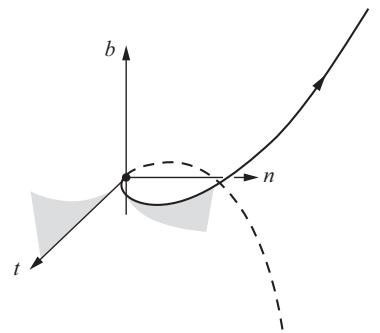
\includegraphics[width=\textwidth]{../../../../PDFs/differential-geometry/transcript/Do Carmo - Differential Geometry of Curves and Surfaces/hybrid_ocr/images/1e6a547641b1e28e3c702fb6e34f46c8a858b466f072c85a849afa6b33da9d72.jpg}}
\newline
\subfloat[投影到 $tb$ 平面]{\label{fig:local-canonical-tb}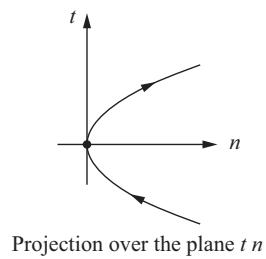
\includegraphics[width=\textwidth]{../../../../PDFs/differential-geometry/transcript/Do Carmo - Differential Geometry of Curves and Surfaces/hybrid_ocr/images/559bd128ff198b162ce66c9ee7c9a939cc608cb17870f0e37b55f457b9d26c95.jpg}}
\newline
\subfloat[投影到 $nb$ 平面]{\label{fig:local-canonical-nb}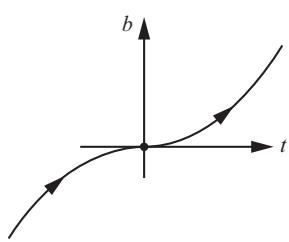
\includegraphics[width=\textwidth]{../../../../PDFs/differential-geometry/transcript/Do Carmo - Differential Geometry of Curves and Surfaces/hybrid_ocr/images/1889978426007c61cdf45a97ae5a1a5a5accffabdac10b46b3f8f73f04ef5f86.jpg}}
\newline
\subfloat[投影到 $tn$ 平面]{\label{fig:local-canonical-tn}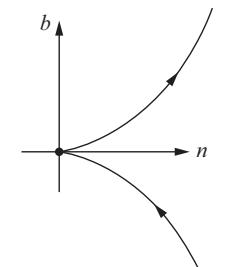
\includegraphics[width=\textwidth]{../../../../PDFs/differential-geometry/transcript/Do Carmo - Differential Geometry of Curves and Surfaces/hybrid_ocr/images/1fb0809e26dc4c3d9b71f6f2f4f516ba37417a1ad2f25349083242b67d20e8fe.jpg}}
\end{minipage}
\end{figure}

\begin{figure}[H]
\centering
\begin{minipage}{0.45\textwidth}
\centering
\subfloat[Figure 1-19 (a). $\tau < 0$ 的情形]{\label{fig:torsion-neg}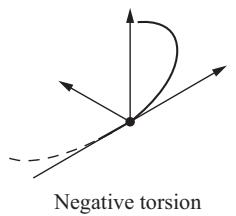
\includegraphics[width=\textwidth]{../../../../PDFs/differential-geometry/transcript/Do Carmo - Differential Geometry of Curves and Surfaces/hybrid_ocr/images/5c650a1fbbf8575a4560f36765774966e5be5ecf980eb69ea5bf1c8af1192924.jpg}}
\end{minipage}
\hfill
\begin{minipage}{0.45\textwidth}
\centering
\subfloat[Figure 1-19 (b). $\tau > 0$ 的情形]{\label{fig:torsion-pos}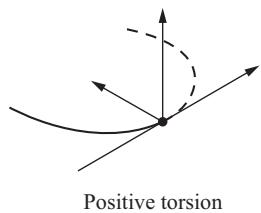
\includegraphics[width=\textwidth]{../../../../PDFs/differential-geometry/transcript/Do Carmo - Differential Geometry of Curves and Surfaces/hybrid_ocr/images/44e707e5ada16aaa4e24604909275fc9a43532bcc6a0e1eebde0ea453c90fee0.jpg}}
\end{minipage}
\end{figure}

\subsection*{1-6 节练习}

\begin{exercise}{1-6, 1}
Write the local canonical form of the helix $\alpha(t) = (a\cos t, a\sin t, bt)$ at $t = 0$.
\end{exercise}

\begin{exercise}{1-6, 2}
Show that the curve $\alpha(s) = (s, \frac{k_0}{2}s^2, \frac{k_0\tau_0}{6}s^3)$ has curvature $k(s) = k_0 + o(s)$ and torsion $\tau(s) = \tau_0 + o(s)$.
\end{exercise}

\begin{exercise}{1-6, 3}
Find the third-order approximation of the curve $\alpha(t) = (t, \sin t)$ at $t = 0$.
\end{exercise}

\begin{exercise}{1-6, 4}
Prove that the osculating circle at a point has radius $1/k$ and center at $\alpha(s) + \frac{1}{k}\mathbf{n}$.
\end{exercise}

\begin{exercise}{1-6, 5}
Show that the osculating circle and the curve have the same tangent direction at the point of contact.
\end{exercise}

\begin{exercise}{1-6, 6}
Find the equation of the osculating circle for the ellipse $\alpha(t) = (a\cos t, b\sin t)$ at $t = 0$.
\end{exercise}

\begin{exercise}{1-6, 7}
Prove that the osculating plane is the limit of the planes through three points $\alpha(s_0)$, $\alpha(s_0 + h)$, $\alpha(s_0 + 2h)$ as $h \to 0$.
\end{exercise}

\begin{exercise}{1-6, 8}
Determine the shape of a curve near a point where $k > 0$ and $\tau = 0$.
\end{exercise}

% ==================== Section 1-7: Global Properties of Plane Curves ====================
\section{Global Properties of Plane Curves}\label{sec:global-properties-ch1}

前面我们讨论的是曲线的局部性质。现在我们讨论平面曲线的整体（全局）性质。

\begin{Definition}[简单闭曲线]\label{def:simple-closed-curve}
一条平面曲线 $\alpha: [0, L] \to \mathbb{R}^2$ 称为\textbf{简单闭曲线}（simple closed curve），如果 $\alpha(0) = \alpha(L)$，且 $\alpha$ 在 $(0, L)$ 上是单射。
\end{Definition}

\begin{figure}[H]
\centering
\begin{minipage}{0.45\textwidth}
\centering
\subfloat[Figure 1-20 (a). 简单闭曲线]{\label{fig:simple-closed}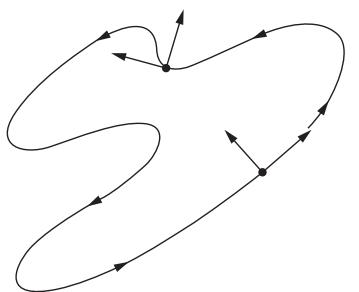
\includegraphics[width=\textwidth]{../../../../PDFs/differential-geometry/transcript/Do Carmo - Differential Geometry of Curves and Surfaces/hybrid_ocr/images/8ea4e8eea7678cad3948cf06b0551ceecf71afff5bf72bb6f76985d606f4722b.jpg}}
\end{minipage}
\hfill
\begin{minipage}{0.45\textwidth}
\centering
\subfloat[Figure 1-20 (b). 非简单闭曲线]{\label{fig:nonsimple-closed}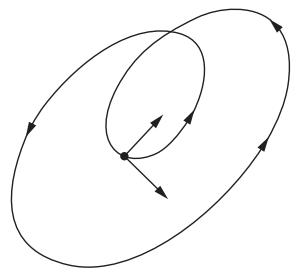
\includegraphics[width=\textwidth]{../../../../PDFs/differential-geometry/transcript/Do Carmo - Differential Geometry of Curves and Surfaces/hybrid_ocr/images/034960a7cc6b6fde35352465512e26d15cc4232f9875e588aab42f7e9fe01290.jpg}}
\end{minipage}
\end{figure}

\begin{figure}[H]
\centering
\begin{minipage}{0.45\textwidth}
\centering
\subfloat[Figure 1-21 (a). 环面上的简单闭曲线]{\label{fig:torus-curve}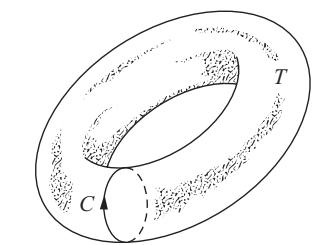
\includegraphics[width=\textwidth]{../../../../PDFs/differential-geometry/transcript/Do Carmo - Differential Geometry of Curves and Surfaces/hybrid_ocr/images/3a2b0c77969ff7631fc9d313f3e38b0d4d65257a4b99a9b9ca75b8e5446ee999.jpg}}
\end{minipage}
\hfill
\begin{minipage}{0.45\textwidth}
\centering
\subfloat[Figure 1-21 (b). 正向定向]{\label{fig:positive-orientation}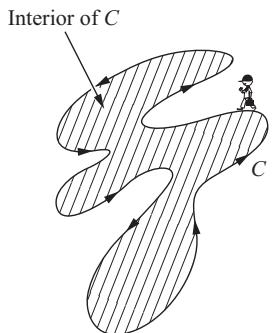
\includegraphics[width=\textwidth]{../../../../PDFs/differential-geometry/transcript/Do Carmo - Differential Geometry of Curves and Surfaces/hybrid_ocr/images/d1fa06b0b42dfa82fca2be8e907ef38765cb5fdc93c76d29bcda32a65eb9f15c.jpg}}
\end{minipage}
\end{figure}

\begin{Definition}[旋转指数]\label{def:turning-number-ch1}
设 $\alpha: [0, L] \to \mathbb{R}^2$ 是一条简单闭平面曲线，参数化为单位速度。定义\textbf{旋转指数}（turning number）为
\[
n = \frac{1}{2\pi} \int_0^L k(s) \, ds.
\]
旋转指数表示切向量沿曲线完整一圈转过的圈数。
\end{Definition}

\begin{Theorem}[旋转指数定理]\label{th:turning-number}
简单闭平面曲线的旋转指数必为整数，且绝对值至少为 $1$。
\end{Theorem}

\begin{Theorem}[四顶点定理]\label{th:four-vertex-ch1}
设 $C$ 是平面上一条简单闭曲线，曲率恒为正。则 $C$ 上至少有四个曲率极值点（顶点）。
\end{Theorem}

\begin{Remark}
"顶点"（vertex）是指曲率取得局部极值的点。四顶点定理是平面曲线理论中最著名的整体定理之一。例如，椭圆有四个顶点（长轴和短轴的端点）。
\end{Remark}

\begin{Theorem}[Fenchel 定理]\label{th:fenchel-ch1}
设 $\alpha: [0, L] \to \mathbb{R}^3$ 是一条简单闭曲线。则其全曲率
\[
\int_0^L k(s) \, ds \geq 2\pi,
\]
等号成立当且仅当曲线是平面上的凸曲线。
\end{Theorem}

\begin{Definition}[全曲率]\label{def:total-curvature-ch1}
曲线 $\alpha$ 的\textbf{全曲率}（total curvature）定义为
\[
\int_0^L k(s) \, ds,
\]
即曲率沿曲线的积分。
\end{Definition}

\begin{Corollary}\label{cor:fenchel-corollary-ch1}
任何简单闭曲线的全曲率至少为 $2\pi$。
\end{Corollary}

\begin{Theorem}[Fary-Milnor 定理]\label{th:fary-milnor-ch1}
如果 $\alpha$ 是一条简单闭曲线的全曲率小于 $4\pi$，则该曲线是未打结的（unknotted）。
\end{Theorem}

\begin{Remark}
这些定理连接了曲线的局部几何（曲率）和全局拓扑性质。四顶点定理说明闭合曲线的"总弯曲量"必须"平衡"；Fenchel 定理说明闭合曲线的全曲率至少是 $2\pi$。
\end{Remark}

\begin{figure}[H]
\centering
\begin{minipage}{0.65\textwidth}
\centering
\subfloat[Figure 1-22. 等周公式证明图示]{\label{fig:fig1-22}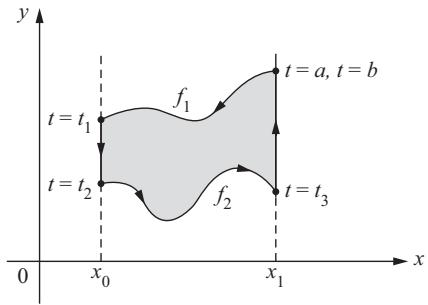
\includegraphics[width=\textwidth]{../../../../PDFs/differential-geometry/transcript/Do Carmo - Differential Geometry of Curves and Surfaces/hybrid_ocr/images/9cfc830e55606447f8926843d144db8601ec13fc42473572cd665be08fc2c5e7.jpg}}
\end{minipage}
\end{figure}

\begin{figure}[H]
\centering
\begin{minipage}{0.45\textwidth}
\centering
\subfloat[Figure 1-23. 等周问题的几何构型]{\label{fig:isoperimetric-config}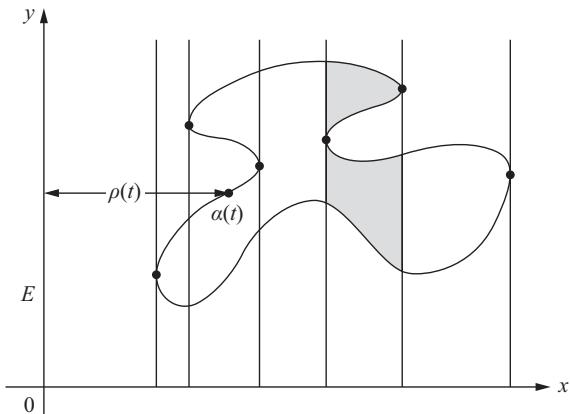
\includegraphics[width=\textwidth]{../../../../PDFs/differential-geometry/transcript/Do Carmo - Differential Geometry of Curves and Surfaces/hybrid_ocr/images/29ac0046be9d030e2d6b0d51c57778a994e77f9712ebe5ac2a3e63401941f75b.jpg}}
\end{minipage}
\hfill
\begin{minipage}{0.45\textwidth}
\centering
\subfloat[Figure 1-24. 等周不等式证明图示]{\label{fig:isoperimetric-proof}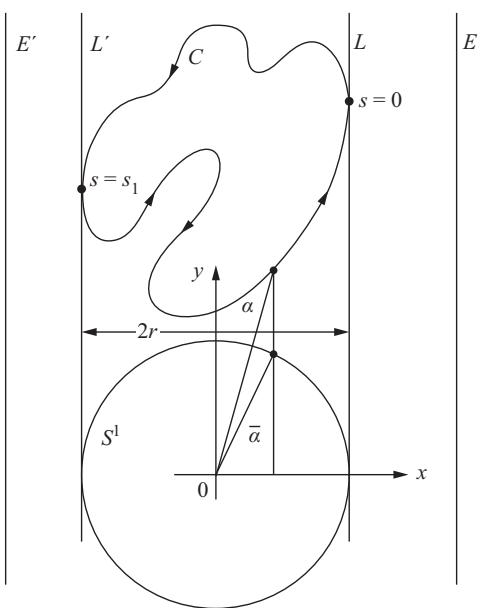
\includegraphics[width=\textwidth]{../../../../PDFs/differential-geometry/transcript/Do Carmo - Differential Geometry of Curves and Surfaces/hybrid_ocr/images/1f888342851bea2237ad4ebb2ceefdc9cdeca51246d624ddcbad61b94698552a.jpg}}
\end{minipage}
\end{figure}

\begin{figure}[H]
\centering
\begin{minipage}{0.6\textwidth}
\centering
\subfloat[Figure 1-25. 分段 $C^1$ 曲线]{\label{fig:piecewise-c1}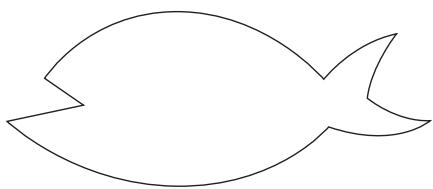
\includegraphics[width=\textwidth]{../../../../PDFs/differential-geometry/transcript/Do Carmo - Differential Geometry of Curves and Surfaces/hybrid_ocr/images/a325c45e4316d76cdb849939f3c5c8e59eeabe101ad105b382b0edef3e23eec6.jpg}}
\end{minipage}
\end{figure}

\begin{figure}[H]
\centering
\begin{minipage}{0.45\textwidth}
\centering
\subfloat[Figure 1-26 (a). 切线指标线]{\label{fig:tangent-indicatrix-a}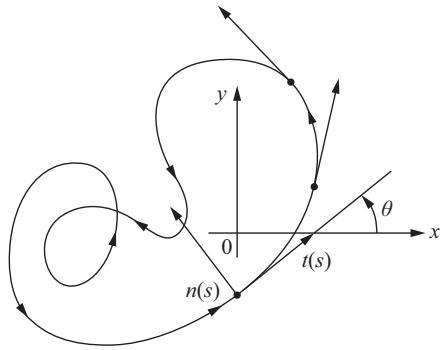
\includegraphics[width=\textwidth]{../../../../PDFs/differential-geometry/transcript/Do Carmo - Differential Geometry of Curves and Surfaces/hybrid_ocr/images/ed8972f41acdd947228696eb1aff57a22d3c79ea04195b25322152a5092b2d99.jpg}}
\end{minipage}
\hfill
\begin{minipage}{0.45\textwidth}
\centering
\subfloat[Figure 1-26 (b). 切线指标线详图]{\label{fig:tangent-indicatrix-b}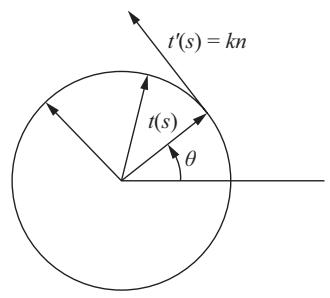
\includegraphics[width=\textwidth]{../../../../PDFs/differential-geometry/transcript/Do Carmo - Differential Geometry of Curves and Surfaces/hybrid_ocr/images/9f5cb3a1ae7c39a5420c6e25848ff8d26636e1a07af4c18bf87cb74dcb14f23d.jpg}}
\end{minipage}
\end{figure}

\begin{figure}[H]
\centering
\begin{minipage}{0.35\textwidth}
\centering
\subfloat[Figure 1-27 (a). 旋转指数为 1]{\label{fig:rotation-index-1}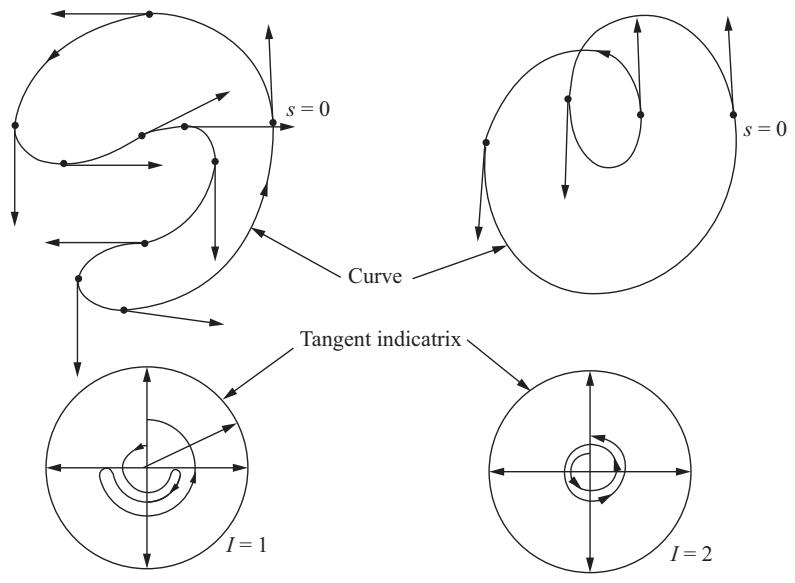
\includegraphics[width=\textwidth]{../../../../PDFs/differential-geometry/transcript/Do Carmo - Differential Geometry of Curves and Surfaces/hybrid_ocr/images/c1056d2b6a48d0190f210c9a7fdeba0fa262e8791d59f8252ee8a071b806c76f.jpg}}
\end{minipage}
\hfill
\begin{minipage}{0.30\textwidth}
\centering
\subfloat[Figure 1-27 (b). 旋转指数为 2]{\label{fig:rotation-index-2}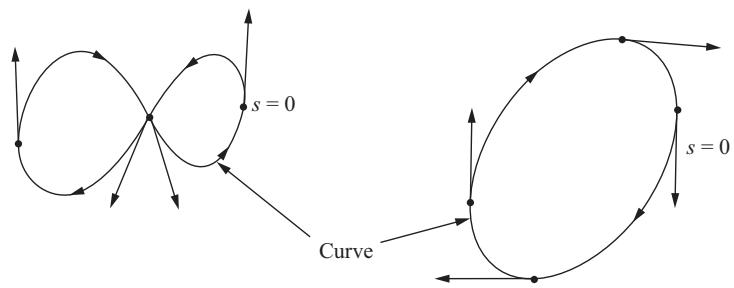
\includegraphics[width=\textwidth]{../../../../PDFs/differential-geometry/transcript/Do Carmo - Differential Geometry of Curves and Surfaces/hybrid_ocr/images/bfcd46a1040027336d83edcb81d47775141684cb0bba7c3dda59703c841db26b.jpg}}
\end{minipage}
\hfill
\begin{minipage}{0.30\textwidth}
\centering
\subfloat[Figure 1-27 (c). 旋转指数为 -1]{\label{fig:rotation-index-neg}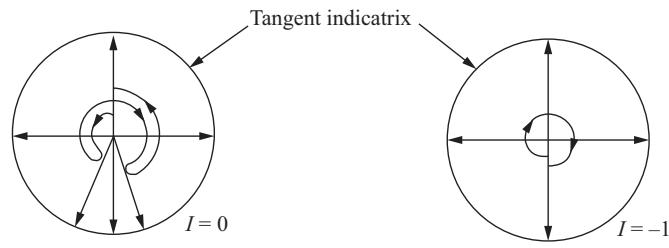
\includegraphics[width=\textwidth]{../../../../PDFs/differential-geometry/transcript/Do Carmo - Differential Geometry of Curves and Surfaces/hybrid_ocr/images/4344fb6535e6e590751cfcb71fc7a04ab9c88b236c3504c6bb25fafcfc9c5319.jpg}}
\end{minipage}
\end{figure}

\begin{figure}[H]
\centering
\begin{minipage}{0.75\textwidth}
\centering
\subfloat[Figure 1-28 (a). 凸曲线]{\label{fig:convex-curve}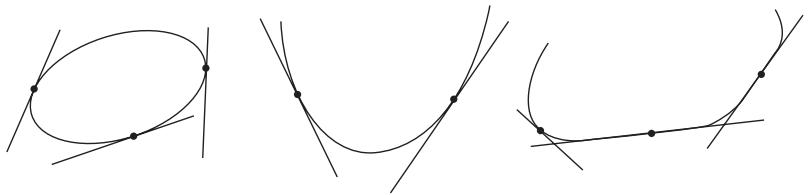
\includegraphics[width=\textwidth]{../../../../PDFs/differential-geometry/transcript/Do Carmo - Differential Geometry of Curves and Surfaces/hybrid_ocr/images/605b716c932cd5e915b8e5296bc4b3e577a93f4c7d7d3fc35e7590742cd5296c.jpg}}
\end{minipage}
\end{figure}

\begin{figure}[H]
\centering
\begin{minipage}{0.70\textwidth}
\centering
\subfloat[Figure 1-28 (b). 非凸曲线]{\label{fig:nonconvex-curve}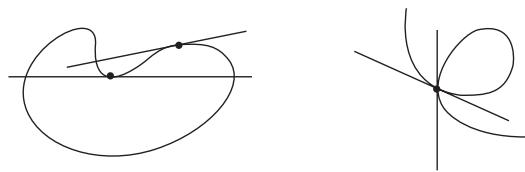
\includegraphics[width=\textwidth]{../../../../PDFs/differential-geometry/transcript/Do Carmo - Differential Geometry of Curves and Surfaces/hybrid_ocr/images/344549a18768464cdc807bdd43ffa550bccfb9852fa5b59672c3d2e70141e497.jpg}}
\end{minipage}
\end{figure}

\begin{figure}[H]
\centering
\begin{minipage}{0.35\textwidth}
\centering
\subfloat[Figure 1-29 (a). 三个不同顶点情况]{\label{fig:four-vertex-a}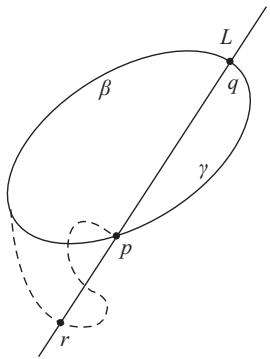
\includegraphics[width=\textwidth]{../../../../PDFs/differential-geometry/transcript/Do Carmo - Differential Geometry of Curves and Surfaces/hybrid_ocr/images/2797eca07f5b8cd6e2426a408534d07b5f1671cf8aa13f28a1b57bab08ecd395.jpg}}
\end{minipage}
\hfill
\begin{minipage}{0.60\textwidth}
\centering
\subfloat[Figure 1-29 (b). 直线段情况]{\label{fig:four-vertex-b}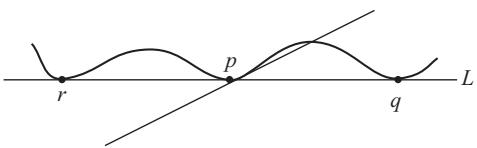
\includegraphics[width=\textwidth]{../../../../PDFs/differential-geometry/transcript/Do Carmo - Differential Geometry of Curves and Surfaces/hybrid_ocr/images/ce7874597bf7b56abe143614c8510607de566ea4819d497bea3b17078bf3fa4f.jpg}}
\end{minipage}
\end{figure}

\begin{figure}[H]
\centering
\begin{minipage}{0.6\textwidth}
\centering
\subfloat[Figure 1-30. 直线族的重数]{\label{fig:line-multiplicity}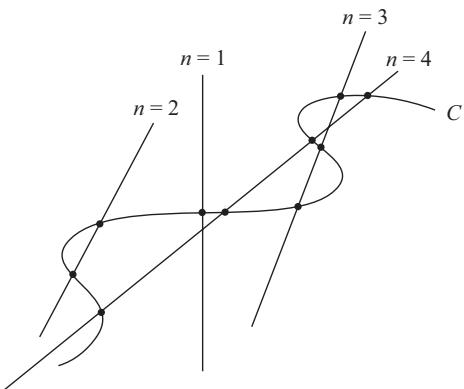
\includegraphics[width=\textwidth]{../../../../PDFs/differential-geometry/transcript/Do Carmo - Differential Geometry of Curves and Surfaces/hybrid_ocr/images/8af60fc93ea0ea82b08ce868637d63a5a839095d24f97b10ab057990e28d0abd.jpg}}
\end{minipage}
\end{figure}

\begin{figure}[H]
\centering
\begin{minipage}{0.6\textwidth}
\centering
\subfloat[Figure 1-31. 直线的参数化]{\label{fig:line-param}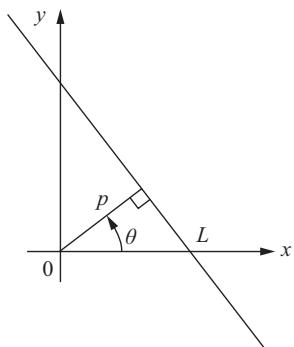
\includegraphics[width=\textwidth]{../../../../PDFs/differential-geometry/transcript/Do Carmo - Differential Geometry of Curves and Surfaces/hybrid_ocr/images/cd4f1bfb9e7c57e2454775fece77bc5393aca16227f9e880341f8709494dea67.jpg}}
\end{minipage}
\end{figure}

\begin{figure}[H]
\centering
\begin{minipage}{0.6\textwidth}
\centering
\subfloat[Figure 1-32. 刚体运动]{\label{fig:rigid-motion}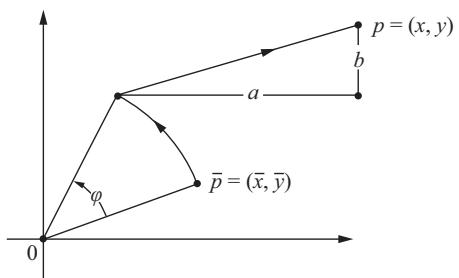
\includegraphics[width=\textwidth]{../../../../PDFs/differential-geometry/transcript/Do Carmo - Differential Geometry of Curves and Surfaces/hybrid_ocr/images/8623bd4bd41d13ccfa7b56b4da654a8467c435e3d691498e94a601f3dafb2ae8.jpg}}
\end{minipage}
\end{figure}

\subsection*{1-7 节练习}

\begin{exercise}{1-7, 1}
Is there a simple closed curve in the plane with length equal to 6 feet and bounding an area of 3 square feet?
\end{exercise}

\begin{exercise}{1-7, 2}
Let $\overline{AB}$ be a segment of straight line and let $l > \text{length of } AB$. Show that the curve $C$ joining $A$ and $B$, with length $l$, and such that together with $\overline{AB}$ bounds the largest possible area is an arc of a circle passing through $A$ and $B$ (见教材 Figure 1-23, 1-24)。
\end{exercise}

\begin{exercise}{1-7, 3}
Compute the curvature of the ellipse $x = a\cos t$, $y = b\sin t$, $t \in [0, 2\pi]$, $a \neq b$, and show that it has exactly four vertices, namely, $(a, 0)$, $(-a, 0)$, $(0, b)$, $(0, -b)$.
\end{exercise}

\begin{exercise}{1-7, 4}
Let $C$ be a plane curve and let $T$ be the tangent line at a point $p \in C$. Draw a line $L$ parallel to the normal line at $p$ and at a distance $d$ of $p$. Let $h$ be the length of the segment determined on $L$ by $C$ and $T$. Prove that $|k(p)| = \lim_{d \to 0} \frac{2h}{d^2}$.
\end{exercise}

\begin{exercise}{1-7, 5}
If a closed plane curve $C$ is contained inside a disk of radius $r$, prove that there exists a point $p \in C$ such that the curvature $k$ of $C$ at $p$ satisfies $|k| \geq 1/r$.
\end{exercise}

\begin{exercise}{1-7, 6}
Let $\alpha(s)$, $s \in [0, l]$ be a closed convex plane curve positively oriented. The curve $\beta(s) = \alpha(s) - r\mathbf{n}(s)$, where $r$ is a positive constant and $\mathbf{n}$ is the normal vector, is called a parallel curve to $\alpha$. Show that:
\begin{enumerate}
\item[a.] Length of $\beta = $ length of $\alpha + 2\pi r$.
\item[b.] $A(\beta) = A(\alpha) + rl + \pi r^2$.
\item[c.] $k_\beta(s) = k_\alpha(s) / (1 + r k_\alpha(s))$.
\end{enumerate}
\end{exercise}

\begin{exercise}{1-7, 7}
Let $\alpha: \mathbb{R} \to \mathbb{R}^2$ be a plane curve defined in the entire real line. Assume that $\alpha$ does not pass through the origin and that both $\lim_{t \to +\infty} |\alpha(t)| = \infty$ and $\lim_{t \to -\infty} |\alpha(t)| = \infty$.
\begin{enumerate}
\item[a.] Prove that there exists a point $t_0 \in \mathbb{R}$ such that $|\alpha(t_0)| \leq |\alpha(t)|$ for all $t \in \mathbb{R}$.
\item[b.] Show, by an example, that the assertion in part a is false if one does not assume both limits are infinite.
\end{enumerate}
\end{exercise}

\begin{exercise}{1-7, 8}
\begin{enumerate}
\item[a.] Let $\alpha(s)$, $s \in [0, l]$, be a plane simple closed curve. Assume that the curvature $k(s)$ satisfies $0 < k(s) \leq c$. Prove that $\text{length of } \alpha \geq 2\pi/c$.
\item[b.] In part a replace the assumption of being simple by "$\alpha$ has rotation index $N$". Prove that $\text{length of } \alpha \geq 2\pi N/c$.
\end{enumerate}
\end{exercise}

\begin{exercise}{1-7, 9}
A set $K \subset \mathbb{R}^2$ is convex if given any two points $p, q \in K$ the segment of straight line $\overline{pq}$ is contained in $K$ (见教材 Figure 1-38). Prove that a simple closed convex curve bounds a convex set.
\end{exercise}

\begin{exercise}{1-7, 10}
Let $C$ be a convex plane curve. Prove geometrically that $C$ has no self-intersections.
\end{exercise}

\begin{exercise}{1-7, 11}
Given a nonconvex simple closed plane curve $C$, we can consider its convex hull $H$ (见教材 Figure 1-39). Use this to show that, in the isoperimetric problem, we can restrict ourselves to convex curves.
\end{exercise}

\begin{exercise}{1-7, 12}
Consider a unit circle $S^1$ in the plane. Show that the ratio $M_1/M_2 = 1/2$, where $M_2$ is the measure of the set of straight lines in the plane that meet $S^1$ and $M_1$ is the measure of all such lines that determine in $S^1$ a chord of length $> \sqrt{3}$ (见教材 Figure 1-40).
\end{exercise}

\begin{exercise}{1-7, 13}
Let $C$ be an oriented plane closed curve with curvature $k > 0$. Assume that $C$ has at least one point $p$ of self-intersection. Prove that:
\begin{enumerate}
\item[a.] There is a point $p' \in C$ such that the tangent line $T'$ at $p'$ is parallel to some tangent at $p$.
\item[b.] The rotation angle of the tangent in the positive arc of $C$ made up by $pp'p$ is $> \pi$ (见教材 Figure 1-41).
\item[c.] The rotation index of $C$ is $\geq 2$.
\end{enumerate}
\end{exercise}

\begin{exercise}{1-7, 14}
\begin{enumerate}
\item[a.] Show that if a straight line $L$ meets a closed convex curve $C$, then either $L$ is tangent to $C$ or $L$ intersects $C$ in exactly two points.
\item[b.] Use part a to show that the measure of the set of lines that meet $C$ (without multiplicities) is equal to the length of $C$.
\end{enumerate}
\end{exercise}

\begin{exercise}{1-7, 15}
Green's theorem in the plane: Let a simple closed plane curve be given by $\alpha(t) = (x(t), y(t))$, $t \in [a, b]$. Assume that $\alpha$ is positively oriented, let $C$ be its trace, and let $R$ be the interior of $C$. Let $p = p(x, y)$, $q = q(x, y)$ be real functions. Then
\[
\iint_R (q_x - p_y) \, dx \, dy = \int_C (p \, dx + q \, dy).
\]
\begin{enumerate}
\item[a.] Set $q = x$ and $p = -y$ and conclude that $A(R) = \frac{1}{2} \int_a^b (x \, dy - y \, dx) \, dt$.
\item[b.] Use Green's theorem to obtain the transformation formula for double integrals.
\end{enumerate}
\end{exercise}

\begin{figure}[H]
\centering
\begin{minipage}{0.3\textwidth}
\centering
\subfloat[Figure 1-38. 凸集定义]{\label{fig:fig1-38}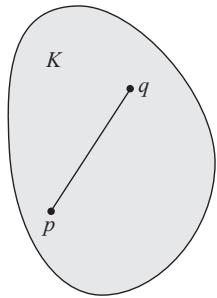
\includegraphics[width=\textwidth]{../../../../PDFs/differential-geometry/transcript/Do Carmo - Differential Geometry of Curves and Surfaces/hybrid_ocr/images/291667aa35426f0fc1ad84813595a255703e09fa4939bf88cba52c32fffc50c4.jpg}}
\end{minipage}
\hfill
\begin{minipage}{0.3\textwidth}
\centering
\subfloat[Figure 1-39. 凸包]{\label{fig:fig1-39}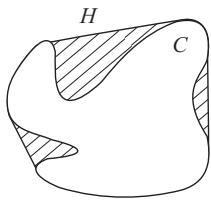
\includegraphics[width=\textwidth]{../../../../PDFs/differential-geometry/transcript/Do Carmo - Differential Geometry of Curves and Surfaces/hybrid_ocr/images/3e78224695b6747abf33b1b0932df3f39b60339272bb783ed8d858be5aadb2c6.jpg}}
\end{minipage}
\hfill
\begin{minipage}{0.35\textwidth}
\centering
\subfloat[Figure 1-40. 单位圆与等边三角形]{\label{fig:fig1-40}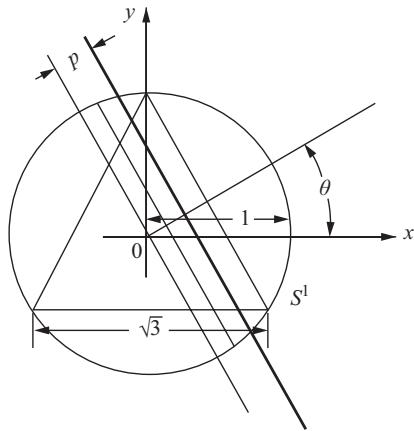
\includegraphics[width=\textwidth]{../../../../PDFs/differential-geometry/transcript/Do Carmo - Differential Geometry of Curves and Surfaces/hybrid_ocr/images/00ec3ddff9ad514cf917444fd074562155a12997a49a644f7ec0989cf7e7d2e8.jpg}}
\end{minipage}
\end{figure}

\begin{figure}[H]
\centering
\begin{minipage}{0.55\textwidth}
\centering
\subfloat[Figure 1-41. 自交曲线旋转角]{\label{fig:fig1-41}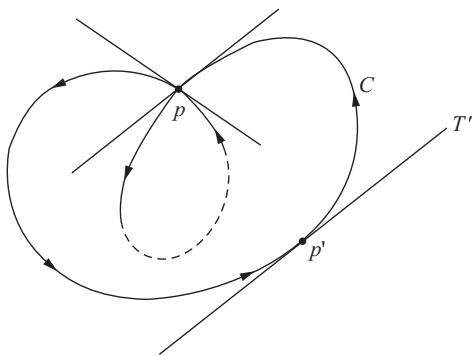
\includegraphics[width=\textwidth]{../../../../PDFs/differential-geometry/transcript/Do Carmo - Differential Geometry of Curves and Surfaces/hybrid_ocr/images/196b87ce5dc9f30daed335b19890a1abf143cb5ea589b33a25641998f788084a.jpg}}
\end{minipage}
\end{figure}

\endinput
